% !TeX program = xelatex
\documentclass[11pt,a4paper]{ctexart}
\usepackage{amsmath,amssymb,bm}
\usepackage[margin=2.2cm]{geometry}
\usepackage{graphicx,booktabs,tabularx,longtable,array}
\usepackage{enumitem,xurl,xcolor}
\usepackage[colorlinks=true,linkcolor=blue!50!black,urlcolor=blue!60!black,citecolor=blue!50!black]{hyperref}
\graphicspath{{plan/unified_gradient_layered_assets/}{unified_gradient_layered_assets/}}
\setlength{\parindent}{2em}
\setlength{\parskip}{0.25em}
\setlist{nosep,leftmargin=2em}
\setlength{\emergencystretch}{2em}
\newcommand{\dd}{\,\mathrm d}
\newcommand{\obs}{\mathsf H_{\mathrm{obs}}}
\newcommand{\wa}{\mathsf W_A}
\newcommand{\btheta}{\boldsymbol\theta}
\title{面向梯度材料高通量表征的\\连续梯度与分层模量统一反演方案}
\author{}
\date{2026年10月22日}

\begin{document}
\maketitle
\begin{abstract}
本研究以梯度材料空间力学性质的高通量表征为目标，针对实际可制备试样主要为分层结构的条件，拟建立同时容纳区内连续变化与跨区模量跳变的二维反演框架。材料场由区域归属函数与局部自由二维场共同描述；数值部分比较现有连续节点方法、分层常值方法和统一方法，实验部分以分层结构验证并与现有方法对照。本文给出参数化、正演、观测及数据项伴随梯度推导，区分先导核验与未完成的识别工作，并规定公平比较、物理验证和表征通量的评价边界。研究先核验表示、积分与梯度，再作小规模无噪声反演诊断；确需稳定化时优先检验仅含一个强度参数的区内梯度正则，复杂的区内／界面联合正则暂缓。该候选尚未实现或验证，数据项推导不等于已经获得稳定的含噪反演算法。
\end{abstract}

\noindent\textbf{状态：}方案与先导核验已形成；统一反演尚未接入当前四步流程，三方法正式对照和新方法的真实DIC识别尚未完成。现有配置、主线数值结果和物理验证状态继续按原协议解释。

\tableofcontents
\newpage

\section{研究目标、科学问题与证据链}
\label{sec:objective}
研究目标是通过一次或少量全场变形实验，可靠获取多个空间位置／材料状态的力学性质，降低逐位置取样与逐组测试的成本。当前制造条件主要支持分层试样，因此以分层结构提供真实实验验证，以连续梯度、分层和混合分布提供数值验证。分层试样是可制造的验证载体；本研究不把目标改成仅识别若干均匀层。

核心问题是：在有限精度和有限空间分辨率的位移观测下，能否用共同的参数化和识别流程，同时恢复区内连续梯度与界面跳变；相对于两类专用表示，增加了哪些可可靠识别的信息，代价和失效条件是什么？

证据链为：高通量空间表征需求 $\rightarrow$ 统一模量表示和反演 $\rightarrow$ 三类数值真值与三方法对照 $\rightarrow$ 分层实物的独立标定和DIC验证。连续梯度与混合分布的结论首先限定为数值能力；分层实验通过不直接等于连续梯度材料已获实验验证。

待检验的贡献包括：
\begin{enumerate}
\item 同一材料表示和参数更新机制覆盖连续、分层及混合分布，不根据最终真值类型切换识别方法。
\item 定量解释连续场对跳变的摊宽偏差、分层常值模型对区内变化的表示偏差，以及统一模型的收益与额外成本。
\item 在保留独立标定、真实载荷和DIC参考约定的条件下，验证分层试样的空间模量识别及重复性。
\item 建立给定精度下的有效空间分辨率和表征通量，区分信息收益、实验节约与求解速度。
\end{enumerate}
上述是研究假设与完成目标，不是当前已证明的结果。

\section{已有基础、相关工作与创新边界}
\subsection{现有项目方法及其局限}
当前反演表示为
\begin{equation}
 E_h(\mathbf x)=\sum_aN_a(\mathbf x)c_a,\qquad c_a=\exp(m_a)>0.
 \label{eq:baseline}
\end{equation}
$N_a$为连续Q4基函数，所有$y$行自由。该表示未预设线性或指数分布，且\textbf{已经允许有限元单元内部模量变化}，但不能表达真正的函数值跳变。当前H1正则为$\gamma\int_\Omega|\nabla E_h|^2\dd A/2$，其平滑倾向与有限元表示限制是不同因素。

既有无噪声合成记录见\path{docs/synthetic_recovery_20261021.md}：分层真值／可表示节点真值的全场模量相对RMS约为2.916\%／2.751\%，七区均值平均绝对偏差约为0.787\%／0.691\%；最终按函数下降停止，未达GTOL。这支持现有方法具备近似分层恢复能力，不支持把真实实验偏差全部归因于界面表示。历史精确TV对照见\path{docs/dic_exact_tv_20261021.md}：既有180N协议下，平均材料标定差异约15.00\%降至14.86\%，未显示实质改善。两者均为已有结果，非统一方法的新结果。

\subsection{与文献的具体关系}
Mei等\cite{mei2024}用B-spline描述界面，以平滑Heaviside组合各区常数剪切模量，联合优化几何与模量；区内均匀是其假设。其不可压缩大变形软组织本构不直接迁移到本项目的小变形平面应力模型。

De Cezaro\cite{cezaro2013}已研究未知界面与区内非恒定参数函数的联合识别。其表示与本方案属于同一类，重点为正则化问题的存在性、稳定性和收敛理论，以及逆势／电磁问题的算法推导；结尾将数值实现列为后续工作。该文不是DIC驱动的梯度材料高通量表征实验，却构成明确的数学先例。不能声称首次提出“未知界面＋区内未知函数”。

graded finite elements早已考虑单元内材料变化\cite{kim2002}；区域限制基函数与Heaviside富集也有成熟基础\cite{noel2022}。连续背景与水平集目标的联合重建见\cite{kadu2017}，但其CT模型及已知异常值条件不同。文献所称“区域／层”和“有限元单元”不能混用。

可主张的新意应集中在\textbf{面向高通量材料表征的统一力学识别能力、具体数值实现及其误差／分辨率规律和实验闭环}，而不是组合公式、链式法则或单元内插值本身。最终优先权判断仍需针对正式实现作进一步文献核查。

\section{统一材料表示与未知量}
\subsection{两区模型的构造}
在$\Omega=(0,L)\times(0,H)$内，以图形界面
\begin{equation}
 x=s(y;\mathbf g),\qquad
 s(y;\mathbf g)=\sum_{\ell=1}^{n_g}b_\ell(y)g_\ell,\qquad
 \phi(x,y;\mathbf g)=x-s(y;\mathbf g)
 \label{eq:geometry}
\end{equation}
区分左右区域。$b_\ell$为已选定的几何B-spline基函数，$g_\ell$为未知横向位置控制量；直界面只需一个位置变量。图形界面限制了可表示拓扑，并不覆盖任意夹杂或界面交叉。

将论文中的区域常数推广为局部二维Q4场：
\begin{equation}
 E_i(\mathbf x;\mathbf m_i)=\sum_aN_a(\mathbf x)c_{ai},
 \qquad c_{ai}=\exp(m_{ai}),\qquad i=1,2.
 \label{eq:branches}
\end{equation}
取$H_\varepsilon(z)=[1+\tanh(z/\varepsilon)]/2$，统一场为
\begin{equation}
 \boxed{E(\mathbf x;\btheta)=[1-H_\varepsilon(\phi)]E_1(\mathbf x)
       +H_\varepsilon(\phi)E_2(\mathbf x),\quad
       \btheta=(\mathbf m_1,\mathbf m_2,\mathbf g).}
 \label{eq:two}
\end{equation}
正模量由非负单位分解和正系数保证；这是充分的系数约束，不等于最一般的域内正值约束。沿用当前数值单位下的对数系数约定，不引入参考模量或目标归一化。$E_i$是先插值正系数，不是$\exp(\sum_aN_am_{ai})$。

$\varepsilon$在$\phi=x-s(y)$方向上具有长度单位。有限$\varepsilon$形成平滑过渡，不能自动解释为物理法向过渡层厚度。尖锐分层由真正的Heaviside表示；有限$\varepsilon$的算法只能称为它的平滑近似。

\subsection{一维例子与三类特例}
令$E_1=a_1+b_1x$、$E_2=a_2+b_2x$，则
\begin{equation}
 E(x)=[1-H(x-s)](a_1+b_1x)+H(x-s)(a_2+b_2x).
\end{equation}
未知量为$(a_1,b_1,a_2,b_2,s)$。两侧系数对应相同得到一条连续直线；$b_1=b_2=0$得到分层常值；两侧斜率与界面差均非零得到区内梯度和跳变；若$a_1+b_1s=a_2+b_2s$但斜率不同，则得到连续折点。

对二维模型，所有分支采用相同系数时，因区域权重和为1，严格恢复式\eqref{eq:baseline}；各区内部系数相同时，因$\sum_aN_a=1$，得到分层常值模型。\textbf{这些关系是空间包含性证明，不是实际反演前施加的系数绑定。}一般反演仍保留独立二维系数，不根据最终真值指定属于哪种特例。

\begin{figure}[htbp]
\centering
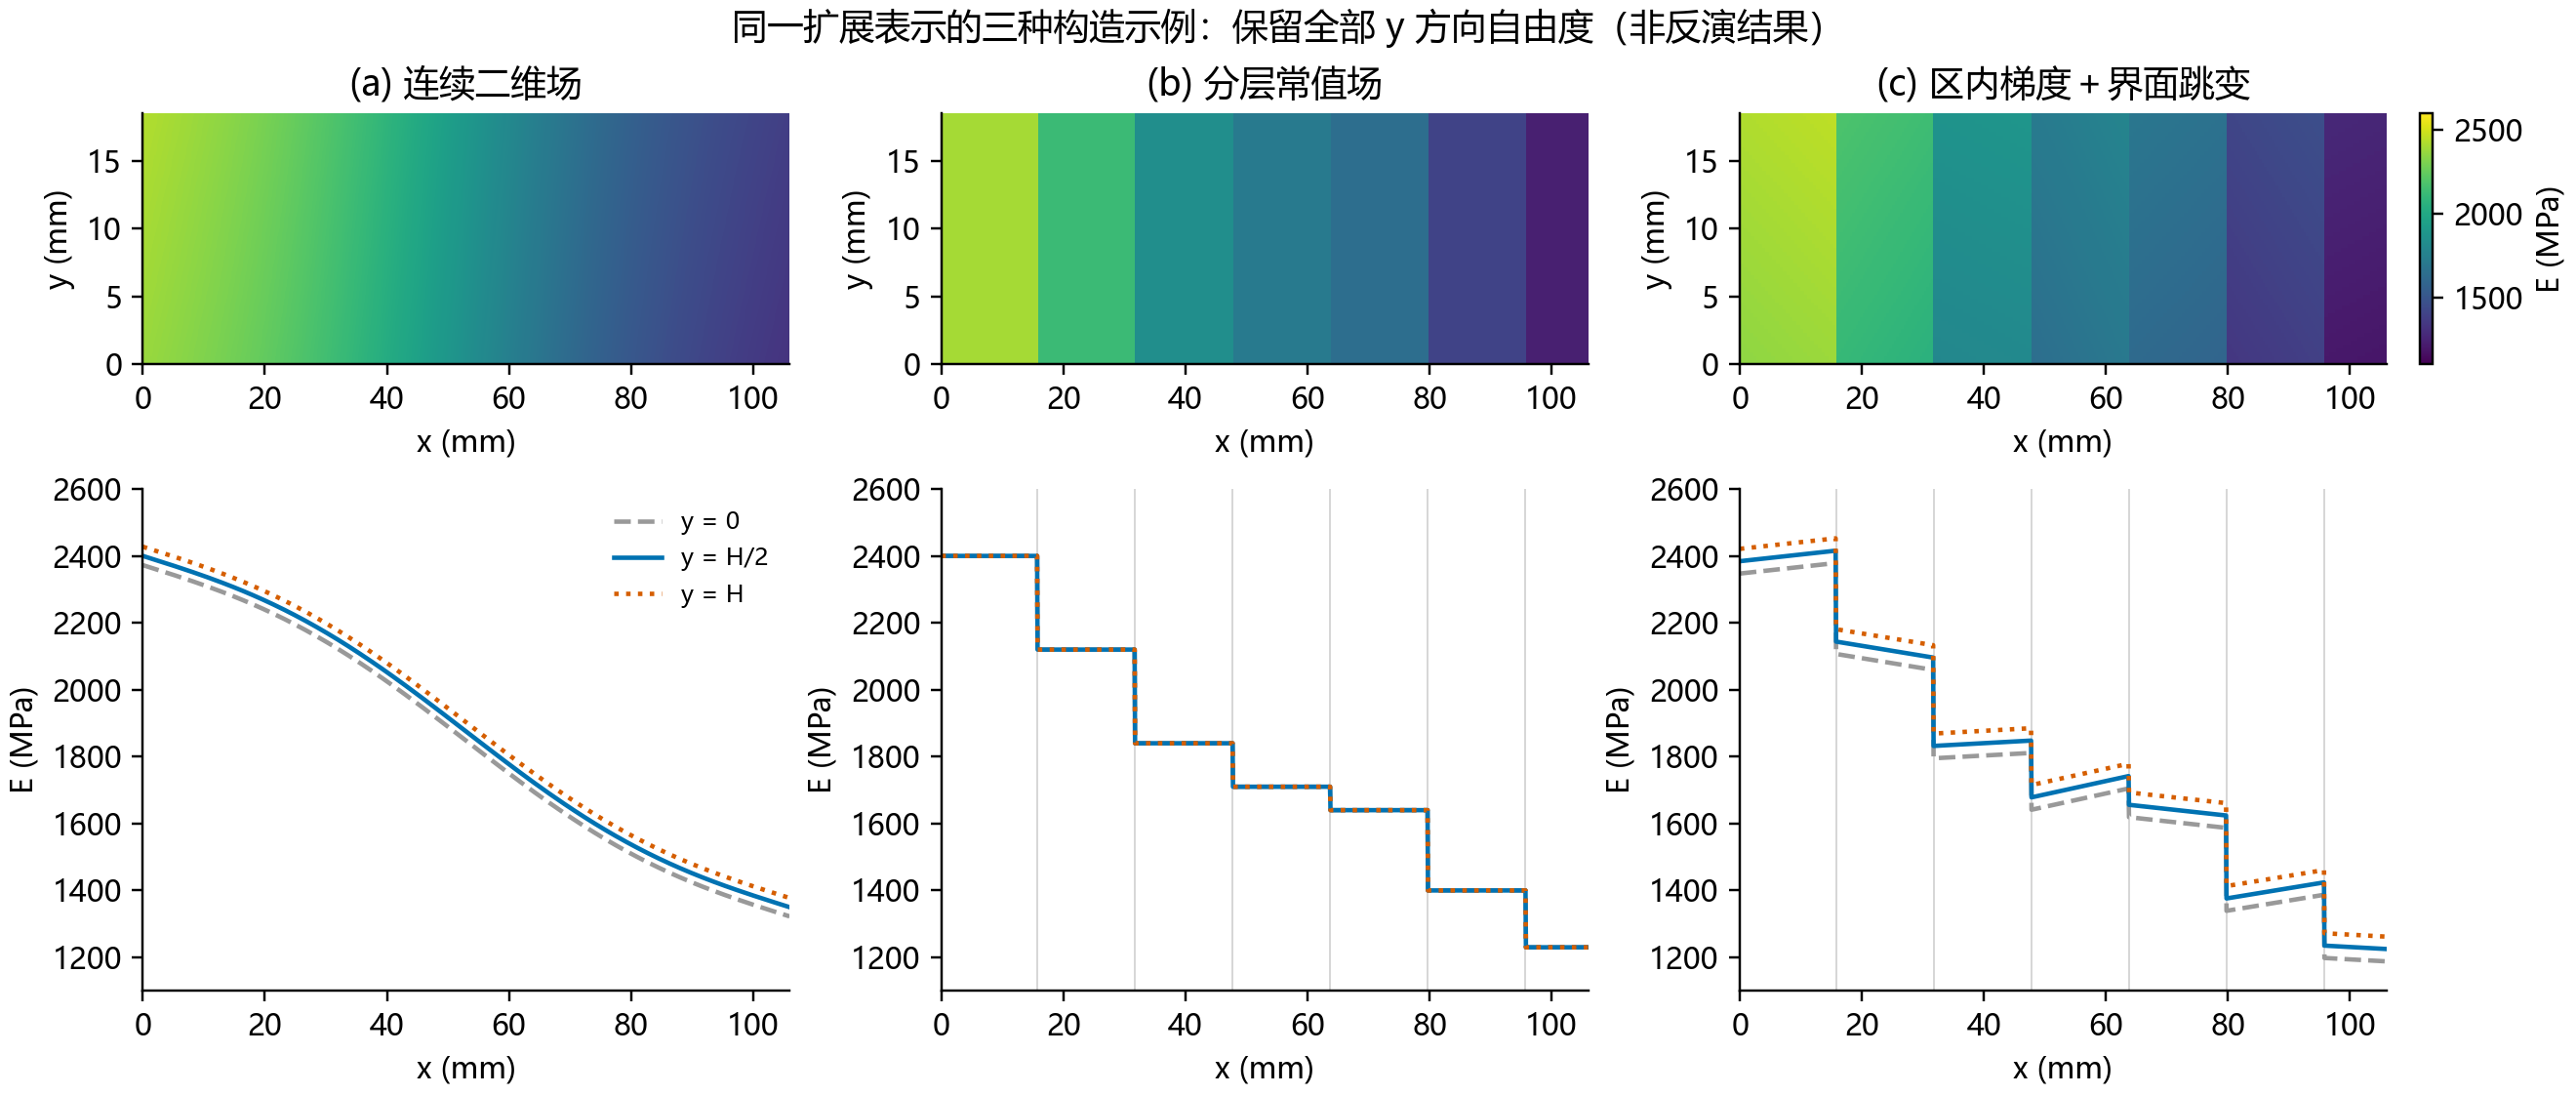
\includegraphics[width=\linewidth]{representation_examples.png}
\caption{同一扩展空间的构造示例。三幅图分别为连续场、分层常值场及区内梯度与界面跳变共存场；全部为人为构造，非反演或实验结果。模型保留$y$方向自由度。}
\end{figure}

\subsection{多区推广及有序界面}
设$K-1$条界面满足$0<s_1(y)<\cdots<s_{K-1}(y)<L$，记$H_j=H_\varepsilon(x-s_j(y))$。采用相同平滑函数和宽度时，定义
\begin{equation}
 \chi_1=1-H_1,\qquad
 \chi_i=H_{i-1}-H_i\ (2\leq i<K),\qquad
 \chi_K=H_{K-1}.
 \label{eq:weights}
\end{equation}
有$\chi_i\geq0$及$\sum_i\chi_i=1$。界面不交叉需要显式可行性约束；对相同非负单位分解几何基函数，逐控制量的严格有序是曲线有序的一种充分条件。不同平滑宽度不能直接沿用非负性结论。

完整表示及等价切换形式为
\begin{align}
 E(\mathbf x;\btheta)&=\sum_{i=1}^{K}\chi_i(\mathbf x;\mathbf g)
                         \sum_aN_a(\mathbf x)\exp(m_{ai}), \label{eq:unified}\\
 &=E_1+\sum_{j=1}^{K-1}H_j(E_{j+1}-E_j). \label{eq:switch}
\end{align}
同一表示可以拟合两类材料，不意味着含噪数据会自动选中准确的连续／跳变结构；尤其不能将“允许跳变”解释为“已识别出真实界面”。

\subsection{哪些量优化，哪些量先规定}
\begin{center}
\small
\begin{tabularx}{\linewidth}{@{}p{0.25\linewidth}XX@{}}
\toprule
量 & 作用 & 本方案中的地位\\\midrule
$m_{ai}$ & 区内模量和二维变化 & 连续优化变量\\
$g_{j\ell}$ & 界面位置／形状 & 未知几何协议下的连续优化变量\\
次数、背景节点与几何节点向量 & 近似精度和分辨能力 & 先规定；不是材料真值\\
候选界面数$K-1$和拓扑 & 允许的结构家族 & 先规定或另作模型选择，不能假称无先验\\
重数、是否插入／删除界面 & 允许的连续性与复杂度 & 离散结构选择，非普通L-BFGS变量\\
$\varepsilon$、步长、停止条件 & 平滑与数值分辨能力 & 数值配置；需敏感性核验\\
初值 & 迭代起点 & 仅由识别数据及声明的几何信息构造，不用真值／标定模量\\
\bottomrule
\end{tabularx}
\end{center}
预设有限维空间是结构假设；给定初值不等于给定最终分布。已知界面和未知界面应分别成协议：前者量化材料表示差异，后者检验几何与模量联合识别。后者不能直接借用真实制造位置作为精确输入。候选界面过多时，零对比界面可能保留为无物理意义的参数，而不代表发现了实际分层。

\section{替代表示及与现有空间的衔接}
\subsection{区域限制基函数与局部富集}
对尖锐固定分区，可用$\chi_iN_a$作为材料基函数，只保留与区域有正面积交集的支撑。远离界面的基函数保留单个系数，跨界面支撑才分裂；这是区域限制／Heaviside富集的材料场实现思路\cite{noel2022}，不要求采用该文全部位移富集或Nitsche条件。

需区分：尖锐固定分区的有效支撑，与式\eqref{eq:unified}的全分支平滑模型。$\tanh$权重具有非紧支撑，不能直接按尖锐活动集丢弃平滑模型的非零项。有限平滑模型的小算例可保留全分支；若采用紧支撑过渡、窄带或域外延拓，需重新证明权重和、正性及参数Jacobian。移动界面还会改变活动集及弱支撑系数的可辨识性。

\subsection{带重复节点的张量积B-spline}
另一实现为
\begin{equation}
 E_h(x,y)=\sum_{a,b}B_{a,p}(x)B_{b,q}(y)c_{ab}.
\end{equation}
次数$p$、内部节点重数$r$对应通常的$C^{p-r}$连续性，$r=p+1$允许函数值跳变；允许不等于强制出现。一次张量积样条与矩形Q4空间相接；在非对齐的直界面处插入两次节点，可保留原连续空间并允许断开。三次样条在重数4处允许跳变，但采用高次区内基函数属于另一个待比较选择。

本项目六个非对齐直界面的先导构造中，粗网格参数量由2440增至2680，细网格由23920增至24700。该计数属于固定直界面的特定一次样条构造，\textbf{不适用于任意曲面、全分支平滑或大范围移动界面}。张量积断线便于当前直分层；弯曲界面更适合区域限制基函数。

\subsection{其他候选及当前取舍}
连续背景与界面目标混合\cite{kadu2017}可迁移到材料场；未经约束的“任意背景＋任意区域修正”可能产生重复表示与相互补偿。参数化水平集可采用紧支撑RBF描述几何，但不自动降低区内材料未知量或消除几何不可辨识性。本阶段优先核验Q4分支与界面组合，样条重复节点作为固定直界面的独立表示核验，不同时引入神经场、任意拓扑搜索或新的复杂正则。

\section{正问题、观测和数据目标}
\subsection{共用平面应力内核}
固定本次计算的泊松比$\nu$，令$\mathsf D(E,\nu)=E\mathsf D_0(\nu)$。按当前单位厚度内核约定，
\begin{equation}
 \mathsf K_e(\btheta)=\int_{\Omega_e}\mathsf B_u^T\mathsf D_0\mathsf B_u
 E(\mathbf x;\btheta)\dd A,
 \qquad \mathsf K(\btheta)\mathbf u=\mathbf f.
 \label{eq:forward}
\end{equation}
厚度一致地进入单位厚度等效载荷，不重复计入。位移基函数和材料基函数是不同角色；材料跳变不要求位移不连续。材料表示准确也不等于当前位移空间已充分解析界面应变变化，仍需正问题网格／积分收敛检查。

对每个识别平台，定义
\begin{align}
 \mathbf r&=\obs\mathbf u+\mathsf R\mathbf c-\mathbf d,\\
 f(\btheta)&=\min_{\mathbf c}\tfrac12\mathbf r^T\wa\mathbf r,
 \qquad \mathbf c_*=(\mathsf R^T\wa\mathsf R)^{-1}
                  \mathsf R^T\wa(\mathbf d-\obs\mathbf u). \label{eq:data}
\end{align}
$\mathsf R$仅含两平移和一微小转动，$\wa$沿用原面积与已声明分量权重。不通过归一化坐标跨度、变形尺度或标定模量改善拟合。

\subsection{先统一表示，再诊断稳定化需求}
本阶段采用以下顺序，\textbf{不把多套正则权重的选择作为表示与实现核验的前提}：
\begin{enumerate}
\item 先核验表示、积分和梯度。这些检查无需选择正则系数，用于确认连续、分层及混合场能否正确表达，以及正演和参数Jacobian是否一致。
\item 用小规模、无噪声、有限预算的反演诊断定位困难，区分区内梯度与界面位置相互补偿、初值敏感、自由度过多和观测信息不足。数据项单独求解用于诊断，不据此保证含噪实验可用。
\item 确有稳定化需求时，优先只保留一个主要正则强度，先检查它是否解决已观察到的问题，再决定是否需要其他机制。
\end{enumerate}

一个待检验的简化候选是
\begin{equation}
 \boxed{\begin{aligned}
 \min_{\mathbf m,\mathbf g}\ J_\gamma(\mathbf m,\mathbf g)
 =f(\mathbf m,\mathbf g)
 +\frac{\gamma}{2}\mathcal R_{\mathrm{intra}}(\mathbf m,\mathbf g),
 \\
 \mathcal R_{\mathrm{intra}}=\sum_{i=1}^{K}
 \int_{\Omega_i(\mathbf g)}|\nabla E_i|^2\dd A.
 \end{aligned}}
 \label{eq:single_gamma}
\end{equation}
数据项$f$仍由式\eqref{eq:data}给出，包含相同的面积权重与三刚体残差配准。该候选沿用原方法抑制空间波动的思路，把平滑约束放在各区域内部，允许区域之间跳变；它是分片梯度惩罚，不是对含跳变的最终全域场计算原H1积分。所有区内$y$行仍独立，不增加材料参考场、界面参考位置惩罚或跳变幅值的独立权重。少量界面位置／形状参数以及有序、不交叉、位于域内等条件优先作为参数化和可行性约束处理。

\textbf{式\eqref{eq:single_gamma}只是优先候选，尚未实现或验证，也未证明足以稳定几何识别。}分层常值场的区内梯度为零，该项不会直接约束其界面位置；连续场的真实斜率仍受惩罚。移动界面使积分域依赖$\mathbf g$，因此正则项的几何导数必须纳入总梯度并独立核验；下节现有公式只给出数据项梯度，不能充当此完整目标的梯度。若采用平滑区域权重近似积分，还需明确其与尖锐分区积分的对应及极限，不能直接改成全域$|\nabla E|^2$。

候选界面数、区内分辨率与平滑宽度仍需规定和检查，减少正则权重不等于没有模型选择。复杂的区内／界面复合正则继续暂缓，不扩展成多参数正则研究。原方法的H1及其L-curve规则保持既有定义；新方法的$\gamma$选择仅使用识别数据，不能直接照搬旧数值或用测试真值／独立标定挑选。正式含噪比较前须明确候选的离散实现、兼容积分、停止与选参规则；未完成时保留未完成状态。

\section{材料参数与界面参数的伴随梯度}
\subsection{材料映射的导数}
对式\eqref{eq:unified}，固定几何时
\begin{equation}
 \boxed{\frac{\partial E}{\partial m_{ai}}=\chi_iN_a\exp(m_{ai}).}
 \label{eq:dm}
\end{equation}
对式\eqref{eq:switch}，利用$\partial\phi_j/\partial g_{j\ell}=-b_\ell(y)$及
\begin{equation}
 H_\varepsilon'(z)=\frac{1}{2\varepsilon}\operatorname{sech}^2(z/\varepsilon),
\end{equation}
得到
\begin{equation}
 \boxed{\frac{\partial E}{\partial g_{j\ell}}
 =(E_j-E_{j+1})H_\varepsilon'(\phi_j)b_\ell(y).}
 \label{eq:dg}
\end{equation}
这些式子假设背景材料基函数和几何基函数已固定，几何仅通过权重进入。若直接优化样条材料节点位置，或改变活动集、坐标映射与积分区域，还需增加相应导数，不能机械套用。

\subsection{消去位移灵敏度}
最优残差配准满足$\mathsf R^T\wa\mathbf r=0$。对固定载荷作参数扰动，有
\begin{equation}
 \delta f=\mathbf r^T\wa\obs\delta\mathbf u,
 \qquad \mathsf K\delta\mathbf u=-(\delta\mathsf K)\mathbf u.
\end{equation}
取与当前代码一致的伴随符号
\begin{equation}
 \mathsf K^T\boldsymbol\lambda=-\obs^T\wa\mathbf r,
\end{equation}
则
\begin{equation}
 \delta f=\boldsymbol\lambda^T(\delta\mathsf K)\mathbf u
         =\int_\Omega S(\mathbf x)\delta E(\mathbf x)\dd A,
 \qquad S=(\mathsf B_u\boldsymbol\lambda)^T\mathsf D_0(\mathsf B_u\mathbf u).
 \label{eq:adjoint}
\end{equation}
代入式\eqref{eq:dm}、\eqref{eq:dg}：
\begin{align}
 \frac{\partial f}{\partial m_{ai}}
 &=\int_\Omega S\chi_iN_a\exp(m_{ai})\dd A, \label{eq:gradm}\\
 \frac{\partial f}{\partial g_{j\ell}}
 &=\int_\Omega S(E_j-E_{j+1})H_\varepsilon'(\phi_j)b_\ell(y)\dd A.
 \label{eq:gradg}
\end{align}
一次正演与一次伴随提供所有参数梯度；每个平台仍只使用自己的识别数据。若单独研究多种独立加载的联合目标，需要另立协议，不能将本方案默认解释为两平台联合拟合。

\subsection{零对比界面与初值退化}
若$E_j\equiv E_{j+1}$，则式\eqref{eq:dg}为零，界面移动不改变材料场或位移；数据不能确定其位置。全部分支从相同均匀初值出发时，几何梯度初始为零是数学性质，不是求导错误。后续能否出现可辨识对比、是否依赖几何初值和是否存在多解，需要受控测试，不能用真实模量初始化规避。

\section{积分、自由度和代码接口的实现边界}
当前\path{fgm_asm/fem_forward.py}的\path{_get_gauss_modulus}在正演中支持材料函数，但当前反演的\path{fgm_asm/inverse_solver.py}中\path{get_stiffness_gradient}仍将高斯点灵敏度映射回原节点系数。正式实现需要共用“参数$\rightarrow$积分点材料值$\rightarrow$Jacobian转置作用”的接口，而不是另复制有限元／伴随内核。

\begin{enumerate}
\item 统一场直接在物理积分点求值。先生成一套全局节点模量再沿旧Q4插值，会重新删除尖锐跳变。
\item 固定尖锐界面采用一致的子区域积分；只在固定高斯点判断区域可能使几何目标呈平台。
\item 有限$\varepsilon$时需解析过渡层，检查积分阶数／细分与$\varepsilon$的耦合。$\varepsilon$减小不能代替积分收敛。
\item 尖锐移动界面需一致形状导数／积分几何导数；式\eqref{eq:gradg}的小平滑验证不替代该项。
\item 活动支撑、小切割区域、域外分支延拓及弱支撑系数可能导致病态；自由度减少、正值限制和预条件均需记录其实际影响。
\end{enumerate}
一个积分反例是单位区间两侧模量为1000／2000，界面从0.3移动到0.6；原两点Gauss积分均为1500，而精确积分由1700变成1400。界面参数虽变化，固定采样未必感知其变化。

后续算法模块仍归\path{fgm_asm/}，数据与报告归\path{lib/}；\path{script/}继续只保留四步入口。本阶段不修改默认配置或接管已有运行。新结果采用独立稳定编号，建议研究根为\path{results/unified_gradient_layered/}；这是计划位置，不表示目录内已有正式结果。

\section{数值对照协议与评价量}
\subsection{三类真值、三种方法}
\begin{center}
\small
\begin{tabularx}{\linewidth}{@{}p{0.17\linewidth}XXX@{}}
\toprule
真值 & 原连续Q4方法 & 分层常值方法 & 统一方法的检验点\\\midrule
连续梯度 & 主要基线 & 阶梯逼近的偏差与所需复杂度 & 保留梯度，抑制虚假界面\\
分层常值 & 界面摊宽及局部幅值偏差 & 强基线，可能更高效 & 恢复幅值和界面，成本合理\\
混合分布 & 跳变表示不足 & 区内梯度表示不足 & 同时识别两种变化\\
\bottomrule
\end{tabularx}
\end{center}
初步数值集合包含缓变／较陡连续场、有限层数的常值场，以及区内非零梯度与跳变共存场；包含适量$y$方向变化以检查自由二维表示，不能因真值一维而绑定反演行。具体幅值、界面、噪声与预算在测试前冻结，先以小网格验证，不直接启动完整网格和大规模参数扫描。

数值识别分成已知界面与未知界面两种协议。已知界面用来隔离材料表示效应；未知界面用来检验几何／材料耦合。两个区域模型获得相同的候选数量和几何信息，不以“新方法已知真实界面、分层法未知界面”制造优势。连续基线本身不使用区域信息，这种表示先验差异应明确报告。

数据、力学模型、观测位置、面积权重、刚体准则、初值来源和硬件一致；按实际总FE计算和耗时统计成本，失败点也计入。不能通过相同$\gamma$数值假称正则强度相同，也不能将更大预算带来的收益全部归因表示。基础对照采用各自明确定义且不依赖测试真值的选参；未完成选参的方法不冒充最优基线。

用于生成最终测试数据的网格／积分应与反演不同，并做参考解收敛检查，减少同表示正反问题自洽造成的有利偏差。另保留同表示核验以检查代码；两者结论不混合。噪声先用固定小算例检验，再覆盖独立种子和相关噪声；选择数据与最终测试数据分离。

\subsection{误差、可辨识性与通量}
共同物理积分下报告
\begin{equation}
 e_E=\sqrt{\frac{\int_\Omega(E_{\mathrm{inv}}-E_{\mathrm{true}})^2\dd A}
                       {\int_\Omega E_{\mathrm{true}}^2\dd A}},
 \qquad
 \mathrm{RMSE}_\alpha=\sqrt{\frac{\sum_k a_k r_{k,\alpha}^2}{\sum_k a_k}},
 \quad\alpha=x,y.
\end{equation}
同时保留完整二维误差、宽度平均$E(x)$、横向空间离散、区均值、界面位置／跳变幅值、界面附近误差和端部误差。横向SD不是参数置信区间；位移拟合好不等于模量唯一。

重点受控变量包括梯度强度、跳变幅度、层厚／过渡尺度、噪声、初值和网格；优先采用少量有判别力的比较，不无条件扩张参数笛卡尔积。可通过灵敏度列相关性、小规模奇异值、扰动恢复及多初值暴露不可辨识性，但不因某个局部Hessian良好就宣称全局唯一。

高通量以\textbf{给定精度与分辨率下获得的有效材料状态数量及其总成本}评价。分别记录实验次数／制样和测量时间、人工介入、计算时间／FE调用、成功率及可解析空间尺度。预先定义误差阈值和状态区分准则后，才可统计可靠状态数$N_{\mathrm{res}}$及每次实验的收益；节点参数数目、像素数或DIC测点数不能直接当作独立材料表征数。统一表示本身不保证计算提速。

\section{分层实验验证及当前项目约定}
实验主对照为统一方法与原连续Q4方法；数值部分保留分层常值强基线。实验只涉及分层结构，不强求为本阶段另制连续梯度试样。独立标定不进入新方法目标、初值或参数选择；界面若由制造资料精确输入，则只能评价已知界面识别，不能再声称盲识别了界面。

沿用\path{plan/validation_plan.md}、\path{post_tensile_test/README.md}和\path{docs/dic_reference_consistency.md}：保留\path{independent}标定的样本数、SD与批次转移限制，不与\path{individual_optimal}混用，不用填充率拟合线替代实测区均值。

当前参考域$105.995084537\times18.484156435$ mm，真实承载宽20 mm、厚3.2 mm。牵引为$F/(20t)$、截取域端力为$FH/20$。FEM $x$沿原始$+Y$，六个材料界面为15.747275、31.747275、47.747275、63.747275、79.747275、95.747275 mm；两端实际覆盖15.747275／10.247810 mm，不是七段均完整16 mm。材料坐标不能按点云重新等分或用识别界面反过来修改物理配准。

180N与280N分别以自身DIC初始化、选参和识别，$\nu\in[0.24,0.33]$、主值0.26；保留当前配置和冻结输入身份，不利用另一平台或标定改选参数。两平台都使用后，本平台回代与跨载荷响应不叫未使用数据验证；比例线弹性载荷不独立增加空间加载模式。

物理坐标、参考态、力配对、横向自由边界近似、完整狗骨与截取域等效和标定转移仍须单独评价。\path{coordinates_verified=false}等现有状态不能因新算法拟合改善自动升级。实验评价包含DIC、独立标定正演和本平台识别回代的同条件双分量对照，以及独立标定模量、识别二维场、$E(x)$和区统计；可靠结论需要独立重复或其他未使用观测支撑。

\section{先导核验、阶段划分与完成标准}
\subsection{已完成的先导记录}
以下小核验发生于正式实现前，保留在\path{plan/unified_gradient_layered_assets/}，不是三方法反演研究结果，也不是独立实验验证。
\begin{enumerate}
\item \path{representation_checks.json}：一次张量积B-spline在当前六个直界面插入两次节点；种子20261022，NumPy 2.4.0、SciPy 1.17.1。原场包含性、七区常值及分段二维仿射场核验的最大绝对误差约$1.4\times10^{-12}$ MPa。原网格为121$\times$19和367$\times$64，扩展参数计数见前文；无反演求解。
\item \path{derivative_checks.json}：$4\times2$单元、$L=4$ mm、$H=1$ mm、$\nu=0.26$、$\varepsilon=0.3$ mm、种子20261022，包含三刚体残差消去，无正则。步长$10^{-5}$下，模量方向／直界面位置的伴随与中心差分相对误差约$9.1\times10^{-10}$／$5.6\times10^{-10}$。两分支相同后，界面改变引起的最大位移变化约$6.5\times10^{-19}$ mm，几何梯度为零。
\end{enumerate}
这些记录保留数值与部分配置，没有完整的独立复现脚本及全部源码身份，不能替代后续正式核验。后续核验需保存配置、版本、命令与依赖源码哈希；按项目约定不长期保留临时测试源码。构造示意图的PNG／SVG同目录保存，不用于误差统计。

\subsection{阶段目标与进入条件}
\begin{description}[style=nextline]
\item[P0：表示、积分和导数]
小规模验证式\eqref{eq:unified}及其Jacobian、正值和权重和、旧连续场严格包含性、零对比几何退化；检查积分阶数／过渡尺度以及尖锐固定界面的子区域积分。这些检查无需正则系数。数学推导与先导记录已形成，正式模块接口和可追溯核验未完成。
\item[P1：最小反演原型]
先在小规模无噪声诊断中比较三类真值，分开固定／未知几何；检查仅由数据构造的初值、多初值和几何退化，定位梯度／界面补偿、初值、过多自由度或信息不足。数据项单独求解只用于诊断。确需稳定化时，优先以式\eqref{eq:single_gamma}的单一$\gamma$候选作小规模检查，先核验其材料和几何总梯度；不自动叠加多套正则。若存在不同场同样拟合、活动集或梯度不一致，保存失败证据并定位，不能用真值初始化或事后约束强行消除。
\item[P2：正式数值对照]
在单参数候选或其他有证据支持的最小稳定化、选参和预算协议明确之后，执行冻结的三方法、三类真值对照；评价独立噪声、表示失配、网格、有效分辨率和通量。新复合正则不属于当前已确定工作内容；数据项诊断或增加一个$\gamma$均不自动代表含噪算法完成。
\item[P3：分层DIC与独立标定]
先完成小规模实现核验，再接入独立研究配置及原四步数据流；按相同输入比较统一场与原连续场，保留平台独立性和物理限制。当前未启动统一方法的大网格扫描或真实实验识别。
\end{description}

每个阶段交付应包含输入／配置、源码版本、随机种子、实际预算、原始场、逐样本指标、停止证据和失败记录。正式结果由独立研究目录保存，不覆盖旧实验、不混入历史TV或其他空间试验的场。

完成标准是形成带范围的结论：统一模型是否扩大了可可靠识别的分布家族；在哪些噪声／梯度／跳变／层厚条件下收益成立或消失；分层实验是否与独立材料证据一致；表征信息收益是否足以抵偿额外成本。允许结论为失败或证据不足，不能用程序运行、优化停止或图形相似替代。

\section{论文定位及尚待解决的问题}
目标论文围绕“有限精度的位移观测中的连续梯度与界面跳变如何共同识别，以及单次试验可可靠获取多少空间材料信息”组织。JMPS可作为冲刺目标，取决于一般性力学表征能力和证据，而非组合公式或期刊先验档位。单次试验识别研究\cite{boddapati2023}、非均匀材料识别研究\cite{salahshoor2026}说明选题相关，但不证明本方案已达发表要求。AMM、IJMS及Experimental Mechanics的匹配度取决于最终方法／力学／实验贡献的侧重，不作录用或分区承诺。

尚待解决：候选界面数量与几何分辨率；平滑模型／尖锐模型及一致积分的选择；几何活动集和弱支撑参数；区内梯度与界面位移相互补偿；稳定化与无真值选参；初值与零对比退化；噪声和有效空间尺度；模型误差与材料真实变化的区分；高通量的可测量收益。当前优先级为P0和P1，不能将这些未知条件隐去后直接宣称统一算法已验证。

\begin{thebibliography}{9}
\bibitem{mei2024} Y. Mei, D. Zhao, C. Xiao, Z. Sun, W. Zhang, X. Guo.
Nondestructively identifying the mechanical behavior of soft tissues using surface deformation with an explicit inverse approach.
\emph{Applied Mathematical Modelling}, 134 (2024), 126--147.
\href{https://doi.org/10.1016/j.apm.2024.05.028}{doi:10.1016/j.apm.2024.05.028}.
\bibitem{cezaro2013} A. De Cezaro.
On a Level-Set Method for Ill-Posed Problems with Piecewise Nonconstant Coefficients.
\emph{Journal of Applied Mathematics}, 2013, 123643.
\href{https://doi.org/10.1155/2013/123643}{doi:10.1155/2013/123643}.
\bibitem{kim2002} J.-H. Kim, G. H. Paulino.
Isoparametric Graded Finite Elements for Nonhomogeneous Isotropic and Orthotropic Materials.
\emph{Journal of Applied Mechanics}, 69(4) (2002), 502--514.
\href{https://doi.org/10.1115/1.1467094}{doi:10.1115/1.1467094}.
\bibitem{noel2022} L. No\"el, M. Schmidt, K. Doble, J. A. Evans, K. Maute.
XIGA: An eXtended IsoGeometric analysis approach for multi-material problems.
\emph{Computational Mechanics}, 70 (2022), 1281--1308.
\href{https://doi.org/10.1007/s00466-022-02200-y}{doi:10.1007/s00466-022-02200-y}.
\bibitem{kadu2017} A. Kadu, T. van Leeuwen, K. J. Batenburg.
A parametric level-set method for partially discrete tomography.
\emph{Discrete Geometry for Computer Imagery}, LNCS 10502 (2017).
\href{https://doi.org/10.1007/978-3-319-66272-5_11}{doi:10.1007/978-3-319-66272-5\_11}.
\bibitem{boddapati2023} J. Boddapati, M. Flaschel, S. Kumar, L. De Lorenzis, C. Daraio.
Single-test evaluation of directional elastic properties of anisotropic structured materials.
\emph{Journal of the Mechanics and Physics of Solids}, 181 (2023), 105471.
\href{https://doi.org/10.1016/j.jmps.2023.105471}{doi:10.1016/j.jmps.2023.105471}.
\bibitem{salahshoor2026} H. Salahshoor, M. Ortiz, L. Stainier.
Data-driven material identification in heterogeneous viscoelastic media.
\emph{Journal of the Mechanics and Physics of Solids}, 213 (2026), 106635.
\href{https://doi.org/10.1016/j.jmps.2026.106635}{doi:10.1016/j.jmps.2026.106635}.
\end{thebibliography}
\end{document}
